\documentclass[12pt]{scrartcl}
\usepackage{listings}
\usepackage{epigraph}
\usepackage{dirtree}
\usepackage{graphicx}


\title{Ideazione progetto e Scelte Implementative}
\subtitle{Ingegneria del Software}
\author{Stefano Ravetta, Simone Renzo, Matteo Scarpone, Mattia Tollari}
\date{29 Febbraio, 2016}

\begin{document}
\maketitle
\centerline{
\includegraphics[scale=0.5]{ITicon.png}}

\tableofcontents
\section{Scelte Implementative}
\subsection{Introduzione}	% Produces subsection heading.  Lower-level subsections
			% are begun with similar \subsubsection and
			% \subsubsubsection commands; numbering is automatic!

\subsubsection{Informazioni su questa sezione del ducumento}
In questa parte di documento verranno trattate e discusse le scelte
implementative che sono state prese per la realizzazione del progetto "Team Diary Management"
e le motivazioni delle stesse .

\subsubsection{Contenuti}
Si porr\`a l'attenzione in modo particolare su
\begin{itemize}
    \item Linguaggio di programmazione
    \item Librerie per la creazione dell'interfaccia utente
    \item Formato e struttura della base di dati
    \item Librerie usate per la gestione del flusso di dati
    \item Struttura dei sistemi di sicurezza adottati
    \item Software per la stesura della documentazione
\end{itemize}

\subsection{Linguaggio di Programmazione}
\subsubsection{Introduzione}
\'E stato scelto il linguaggio di programmazione Python\footnote{https://www.python.org/} per alcune caratteristiche
piuttosto interessanti che lo possono far risaltare nell'ecosistema dei linguaggi di programmazione odierno.
\subsubsection{Alto livello}
Python consente di programmare ad un livello molto alto: con poche righe riesce a gestire
in modo semplice e diretto operazioni complesse senza che il codice risulti troppo complesso da leggere e comprendere.
\\ \\
Questo ha permesso al team di sviluppo di concentrarsi maggiormente sulle parti pi\`u astratte
e progettuali (come i design pattern e la rimozione di vari code smell) rispetto
a questioni pi\`u vicine alla comprensione del funzionamento del linguaggio.
\subsubsection{Filosofia}
Una parte di un famoso "easter egg"\footnote{Questo easter egg, "The Zen of Python"
\`e stato inserito nell'interprete Python e che pu\`o apparire appena si prova ad 
importare la libreria "this".
}
recita:
\begin{quotation}
If the implementation is hard to explain, it's a bad idea.
\end{quotation}

\begin{quotation}
If the implementation is easy to explain, it may be a good idea.
\end{quotation}
Queste righe sembrano denotare con toni sarcastici la filosofia del linguaggio.
Uno degli obiettivi del linguaggio \`e appunto far s\`i che il codice scritto
risulti il miglior compromesso tra stringatezza e comprensibilit\`a. Si intende,
quindi, che codice estremamente compatto non \`e sinonimo di efficienza a lungo termine
in quanto provocher\`a quasi sicuramente un dilatamento delle tempistiche
sia in fasi di sviluppo successive, sia in fase di testing ed ottimizzazione.
Un esempio che pu\`o far notare il modo in cui questo tipo di filosofia inserito
nella struttura del linguaggio possa effettivamente influire sul codice \`e 
quello dell'indentazione: per forzare il programmatore ad indentare sempre
il codice (e a farlo in modo corretto) questo linguaggio non usa caratteri
di begin ed end nella definzione di classi, espressioni condizionali,
espressioni iterative, funzioni e procedure (come fa ad esempio Java con le
parentesi graffe) ma usa solo l'indentazione. In tal modo, da una parte i programmatori
che di norma non indentano il loro codice risulteranno "costretti" a farlo,
e dall'altra i programmatori che gia` di norma indentano il proprio codice
non dovranno inserire altri simboli per esprimere ci\`o che concettualmente
pu\`o essere gi\`a espresso dall'indentazione. \\ \\
Secondo il nostro team di sviluppo, questa caratteristica risulta molto
interessante per la gestione di un progetto in cui \`e richiesta
particolare attenzione alla qualit\`a del codice prodotto. Inoltre, a livello
pratico, tutto ci\`o \`e risultato addirittura comodo perche` si \`e mostrata la
necessit\`a di lavorare con uno stile di stesura del codice unico (ogni membro
del gruppo ne presentava uno diverso).

\subsubsection{Portabilit\`a}
Python \`e un linguaggio precompilato e il suo interprete \`e disponibile per
numerose\footnote{L'elenco delle piattaforme supportate \`e reperibile a https://www.python.org/download/other/} piattaforme. 
La presenza di questa caratteristica non \`e stata sicuramente
ignorata dato che quasi tutti i membri del team di sviluppo usano piattaforme ed ambienti
diversi. Anche la distribuzione dell'applicazione e di pacchetti contenenti le 
varie dipendenze risulta estremamente semplificata grazie alla portabilit\`a di Python.


\subsubsection{Dizionari}
Una delle funzionalit\`a che sono state pi\`u apprezzate per la stesura del codice
relativa al progetto \`e senza dubbio la gestione dei dizionari che Python offre
e la loro semplice e diretta interazione con classi e anche dati Json.


\subsection{Librerie per la creazione dell'interfaccia utente}
\subsubsection{Introduzione}
Sono state scelte le librerie Qt\footnote{http://www.qt.io/} che fanno parte di uno storico
framework open source. 
\subsubsection{Potenzialit\`a}
Le librerie Qt sono in grado di gestire interfacce grafiche, basi di dati, 
attivit\`a multimediali, flussi di rete, gestione di file e notifiche di sistema.
Una caratteristica piuttosto interessante di queste librerie \`e che possono essere usate
attraverso molti\footnote{\`E possibile visionare tutti i linguaggi supportati a questa pagina: 
http://wiki.qt.io/Category:LanguageBindings}
linguaggi di programmazione e non sono legate a nessuna piattaforma specifica.
Permettono anche lo sviluppo di applicazioni mobile\footnote{
il progetto SailfishOs pu\`o dare un'idea delle potenzialit\`a delle librerie Qt:
http://sailfishos.org/develop/sdk-overview/}
\subsubsection{Ambienti di sviluppo}
Per lo sviluppo dell'interfaccia grafica \`e stato comodo usare lo strumento
QtDesigner\footnote{http://doc.qt.io/qt-4.8/designer-manual.html} (che segue il paradigma WYSIWYG) 
che permette di disegnare GUI, modificare le propriet\`a dei vari
oggetti e generare codice XML dell'interfaccia realizzata.
\subsubsection{interazione con Python}
Per far interagire il file XML generato da QtDesigner con Python
\`e stato usato lo strumento Pyuic4\footnote{http://pyqt.sourceforge.net/Docs/PyQt4/designer.html}
che svolge il lavoro meccanico di conversione da file che descrive un'interfaccia
ad uno script Python che mette a disposizione classi che rappresentano
gli oggetti usati ed i metodi  per accedervi. \\ \\
Le librerie Qt sono inoltre state usate sulla parte server per implementare una
gestione dei thread.

\subsection{Base di dati}
\subsubsection{Introduzione}
    Dato che la base di dati usata ha una struttura molto semplice \`e stato scelto
    di non usare uno strumento complesso come un database relazionale. 
    \`E stata creata una base di dati in formato Json che \`e risultata semplice da
    strutturare e da gestire. \`E risultato comodo interagire assieme sulla base
    di dati tramite Git. L'unico problema riscontrato \`e stato dover gestire i vari
    file dal codice dell'applicazione. Questo problema \`e stato praticamente risolto
    con l'introduzione di una struttura di metodi e costanti.
    Con un database relazionale sarebbe stato necessario usare
    i file ottenuti dal dump del database ed importarli in locale ad ogni modifica.
    L'ideazione e la gestione del database relazionale avrebbero occupato pi\'u tempo
    della soluzione adottata.
\subsubsection{Struttura}
    La struttura della base di dati \`e cos\`i definita:
    
    \dirtree{%
    .1 database.
    .2 user.json.
    .2 location.json.
    .2 activity.json.
    .2 group.json.
    .2 project.json.
    }
    
        \underline{User.json}\\
        Contiene i dati relativi all'utente: id, username, password, nome, cognome, gruppi (una lista che
        contiene l'id del gruppo e il ruolo ("partecipante" o "team leader"), vacanze (una listas che
        contiene un id, un nome, data di inizio e data di fine).\\
    
    \underline{Location.json}\\
        Contiene i dati relativi ai luoghi: un id ed un nome.\\
    
    \underline{Activity.json}\\
        Contiene i dati relativi alle attivit\`a: id, nome, id del progetto di riferimento, 
        id dell'utente che ha creato l'attivit\`a, tipo di attivit\`a (se di gruppo, di progetto
        o singola), l'id del luogo, id del grupppo, lista di id dei partecipanti.\\
    
    \underline{Group.json}\\
        Contiene i dati relativi ai grupi: id, nome, father (False se il gruppo non \`e un sottogruppo,
        id del sottogruppo altrimenti), lista degli id dei sottogruppi.\\
        
\subsubsection{Interazione con Python}
    Per importare e gestire la base di dati dal programma sono stati usati i dizionari costruiti,
    come Json, con [chiave: valore]. Questo tipo di dato ha reso molto agile
    l'accesso e la generazione di codice Json.

\subsubsection{Librerie usate per la gestione del flusso di dati}
\`E stato scelto di usare la libreria Flask\footnote{http://flask.pocoo.org/} che permette
una semplice implementazione delle REST Api. \`E stato scelto questo strumento in quanto
risulta avere una curva d'apprendimento leggera. Ha meno funzionalit\`a di altre soluzioni,
ma per le il progetto implementato era pi\`u che sufficiente. Questo ha comunque reso
il pacchetto software finale pi\`u leggero e pi\`u reattivo.

\subsection{Struttura dei sistemi di sicurezza adottati}
\subsubsection{Codifica delle password}
    Per evitare di salvare le password degli utenti in chiaro
    \`e stato fatto ricorso ad un algoritmo di hashing one-way:
    esiste una funzione semplice da calcolare che associa ad ogni stringa un hash
    ma non esiste una funzione semplice da calcolare che associa ad ogni hash una stringa
    tale che, se applicata la funzione iniziale, l'hash ottenuto sia quello di partenza.
    \`E stato scelto SHA512 in quanto oggi risulta quello pi\`u robusto a 
    livello di problemi di collisione e preimmagine. Per l'implementazione in Python
    \`e stata usata la libreria Hashlib.
\subsubsection{Token, autenticazione e gestione delle sessioni}
    Per gestire autenticazione e sessioni \`e stato implementato un sistema di
    token. Un token \`e un hash SHA512 di utente, password e timestamp. Con un controllo
    su questi tre campi si impedisce ad un utente malintenzionato (che non dispone dei una
    password valida) di poter accedere ad una sessione gi\`a attiva. 
    Il timestamp serve per imporre scadenze al token (limite attualmente posto
    uguale ad un giorno). Cos\`i facendo risulter\`a difficile anche provare un
    attacco che mira a scoprire il token dato che in poco tempo i tentativi precedenti
    risulteranno inutili.
\subsubsection{Password dimenticate}
    Nel caso venisse smarrita la password di un utente verr\`a visualizzato
    un messaggio che indicher\`a di contattare gli amministratori di 
    sistema. \`E stata presa questa scelta perch\`e non erano presenti
    le risorse necessarie per implementare e testare a fondo un sistema
    di recupero password che usi email o SMS.

\subsection{Software per la stesura della documentazione}
\subsubsection{Testi}
    \`E stato scelto di usare \LaTeX perch\`e lavorare su file di testo \`e molto
    comodo (anche per quanto riguarda l'uso di Git). Inoltre offre numerose
    funzionalit\`a utili e semplici da gestire per impinazione, gestione paragrafi
    e adattabilit\`a dello stile.
\subsubsection{Diagrammi}
    Per il disegno dei diagrammi \`e stato usato il software "Visual Paradigm";
    \`e in grado di strutturare diagrammi di classi, sequenza, attivit\`a e
    stato in modo piuttosto elegante.

\section{Ideazione del progetto}
\subsection{Obiettivi del progetto}
Il cliente richiede un sistema di gestione e controllo del flusso
di lavoro con relative agende per i progetti di sviluppo software.

Il sistema permette di mantenere aggiornate le attivit\`a per ogni
singolo progetto, ogni gruppo di lavoro gestito da un Team Leader
e ogni sviluppatore che intende pianificare attivit\`a individuali.

La gerarchia delle utenze che possono utilizzare il sistema parte
dal Project Manager, figura con la responsabilit\`a completa di uno
o pi\`u progetti, passando per il Team Leader a capo di uno o pi\`u
gruppi di lavoro all'interno di un progetto fino al singolo
sviluppatore, denominato partecipante, con il set pi\`u ristretto
di operazioni.

\subsection{Introduzione a Manageit}
La soluzione sviluppata, denominata ManageIT, permette di integrare
al meglio le richieste del cliente mantenendo una scalabilit\`a costante
ed un alto livello di estensibilit\`a.

Il software si presenta in versione multipiattaforma, 
utilizzante tecnologie open source
e a basso impatto sul sistema.

Le funzionalit\`a implementate comprendono:
\begin{itemize}
\item Sistema di login sicuro con crittografia SHA-512
\item Gestione integrata dell'agenda di progetto
\item Sistema di gerarchia utenza con permessi dedicati
\item Notifiche alla modifica di dati in modo distribuito
\item Controllo dei vincoli e delle collisioni dei dati
\end{itemize}

L'usabilit\`a \`e garantita da un'interfaccia
grafica semplice, che presenta tutte informazioni di interesse, dotata di
sistemi che evitano operazioni non consentite. Il tutto usa particolari
librerie grafiche multipiattaforma dal design piacevole ed
uniforme.

Le visualizzazioni principali includono il login iniziale,
la presentazione d'agenda generale con varie operazioni
effettuabili e le sotto-sezioni dove aggiungere, modificare o
cancellare dati. Vegono gestite sia attivit\`a individuali, di gruppo o progettuali.
Il sistema non integra
un automatismo per recuperare le credenziali in modo da prevenire
attacchi alla base di dati che dovr\`a essere direttamente gestita
dal Database Manager dell'azienda in questione.

\subsection{Analisi dell'Architettura Software}
ManageIT \`e un sistema basato su interazione Client - Server, strutturato
in modo da poter lavorare anche in modalit\`a offline.

La parte server \`e ampliamente configurabile ed estendibile e non \`e dipendente
da base di dati e sistema di login.
L'interfaccia \`e resa inoltre indipendente dal sottosistema di controllo,
permettendo cos\`i un mantenimento pi\`u veloce e una migliore adattabilit\`a
alle possibili esigenze future.

\subsection{Design Patterns}
\subsubsection{Observer}
    Nella progettazione dell'interfaccia grafica sono stati sfruttati
    componenti ad eventi: il sottosistema inizializza la GUI e si registra
    come ascoltatore di alcuni eventi della stessa attivando quindi 
    determinati metodi solo all'utilizzo di tali componenti.\\
    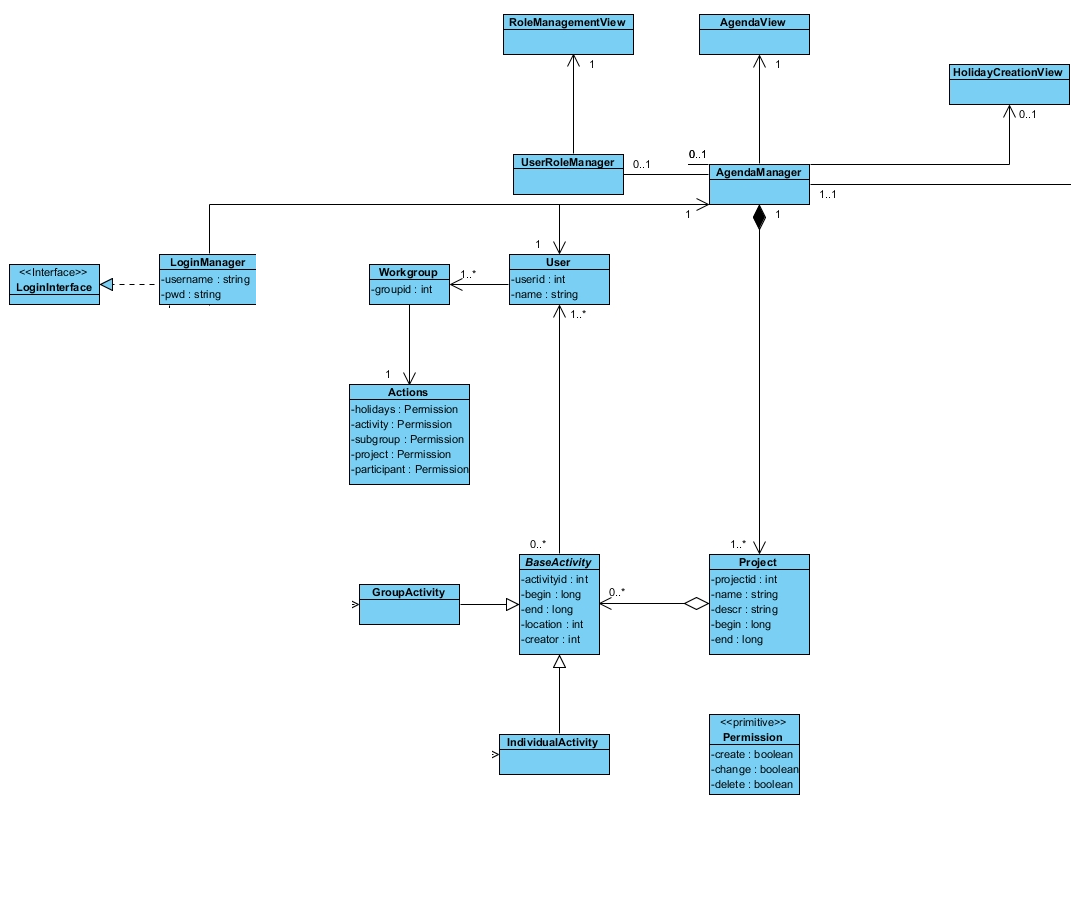
\includegraphics[scale=0.40]{0.png}
Il vantaggio di questo Design Pattern risiede nell'evitare eventi
periodici di controllo della interfaccia grafica mediante polling,
risparmiando quindi grandi quantit\`a di risorse di calcolo e mantenendo
pi\`u leggero e reattivo il software sviluppato.

A livello di accoppiamento inoltre il gestore sottostante conosce
la parte di GUI a cui \`e collegato ma non avviene il contrario, 
permettendo cos\`i la sostituzione veloce di parti di interfaccia
in base alle esigenze. Inoltre se necessario pi\`u classi possono
ascoltare eventi dalla stessa sezione di GUI senza dover modificare
la stessa che diffonde i suoi eventi a tutti gli ascoltatori.
\subsubsection{Facade}
Il Design Pattern denominato Facade \`e stato utile per dividere
in modo efficace i singoli sottosistemi dei package individuati
permettendo una facile comunicazione tra di loro senza aumentare
il numero di accoppiamenti tra classi diverse.\\
    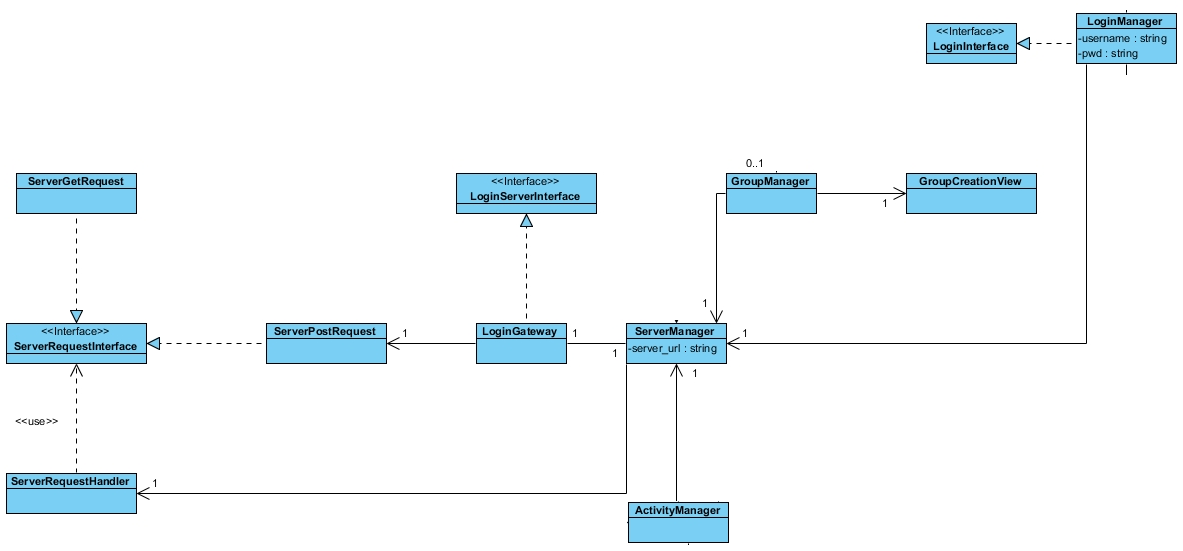
\includegraphics[scale=0.40]{1.png}
Nel progetto in questione il pattern \`e stato sfruttato in modo
semplificato in tutti i package ad esclusione della GUI dove
non \`e previsto. In particolare le chiamate ai package destinati
al networking o allo storage dei dati vengono interamente filtrate
e smistate da classi dedicate che sono appunto le Facade individuate.

Tra i vantaggi di questo pattern troviamo sicuramente una riduzione
dell'accoppiamento tra classi, un maggiore riutilizzo di un sottosistema
o package del sistema che pu\`o quindi essere interfacciato facilmente
con altri sistemi senza reimplementare intere classi ed inoltre non
esclude la possibilit\`a all'utente di accedere direttamente al
sistema "nascosto" che rimane a tutti gli effetti visibile ed
usabile nel modo che si ritiene opportuno.
\subsection{Architectural Patterns}
\subsubsection{Remote Facade}
Il pattern in questione rientra nella categoria architetturale e pu\`o
essere visto come una estensione del precedente Facade applicato per\`o
in ambito di networking. In questo caso la classe che funge da Remote
Facade permette di aggregare pi\`u operazioni che necessitano di connessione
di rete per essere eseguite riducendo cos\`i l'overhead, il traffico,
la congestione e la latenza della richiesta stessa.\\
    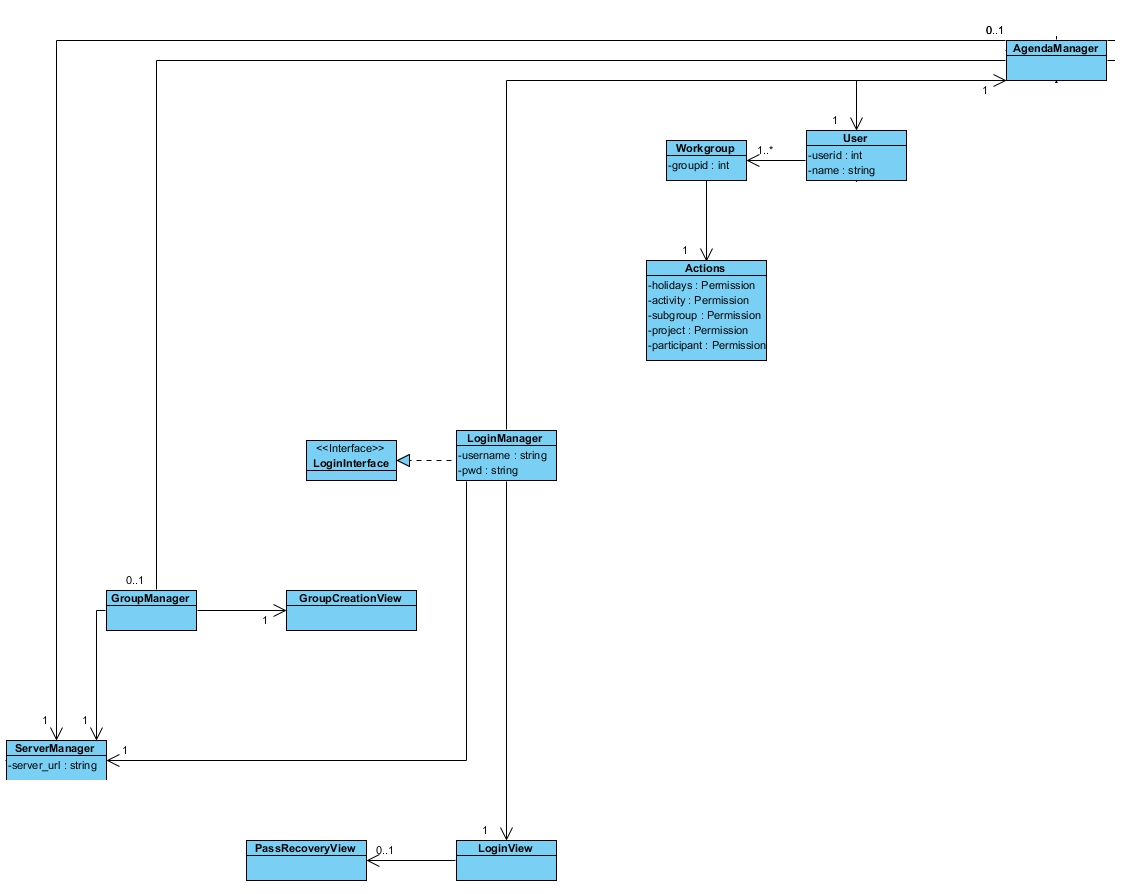
\includegraphics[scale=0.40]{2.png}
Il funzionamento del Remote Facade comprende il ricevere dati da diverse
classi o da diversi attributi/metodi di una classe, raggrupparli in un unico
metodo che creer\`a la richiesta web unificata senza inviarli singolarmente.
Nel progetto \`e stato utilizzato in diverse casistiche tra cui il sistema
di login oppure le operazioni che comprendono creazione di contenuti.
Il pattern inoltre viene comunemente utilizzato, seppur in modo diverso,
nella progettazione di API RESTful che permettono di far risaltare al meglio
questo tipo di pattern.

\subsubsection{Gateway}
Durante la creazione di classi Facade ci si pu\`o confondere con un pattern
architetturale denominato Gateway che sostazialmente fornisce un sistema
simile ma risolve un problema affine. Infatti il pattern Gateway permette
di semplificare l'accesso ad una determinata interfaccia impacchettando le operazioni
necessarie ad effettuare quella di interesse. \\
    \includegraphics[scale=0.6]{3.png}
Un altro vantaggio da non sottovalutare risiede nella semplicit\`a di testing
di una classe Gateway rispetto ad utilizzare una interfaccia complessa o pi\`u
classi correlate, rendendo quindi il controllo del software pi\`u veloce ed efficace.
Il sistema sfrutta questo pattern nell'interfacciamento con il sistema di Database
sottostante, essendo sviluppato in modo da semplificare le query ed aggregarle in
semplici operazioni richiamabili dalle classi che ne necessitano l'accesso.

\subsubsection{Separated Interface}
Durante la progettazione del sistema software ci si \`e concentrato sullo sviluppare
una architettura che potesse supportare al meglio qualsiasi tecnologia utilizzata
riguardo i sistemi di Login o di storage di dati in Database.
Per separare l'implementazione dalla interfaccia per utilizzarla viene in aiuto
il pattern Separated Interface che prevede la definizione di una interfaccia
comune e separata in un altro package (non nel nostro caso, per la natura di Python)
implementata poi nel modo pi\`u conveniente.\\
    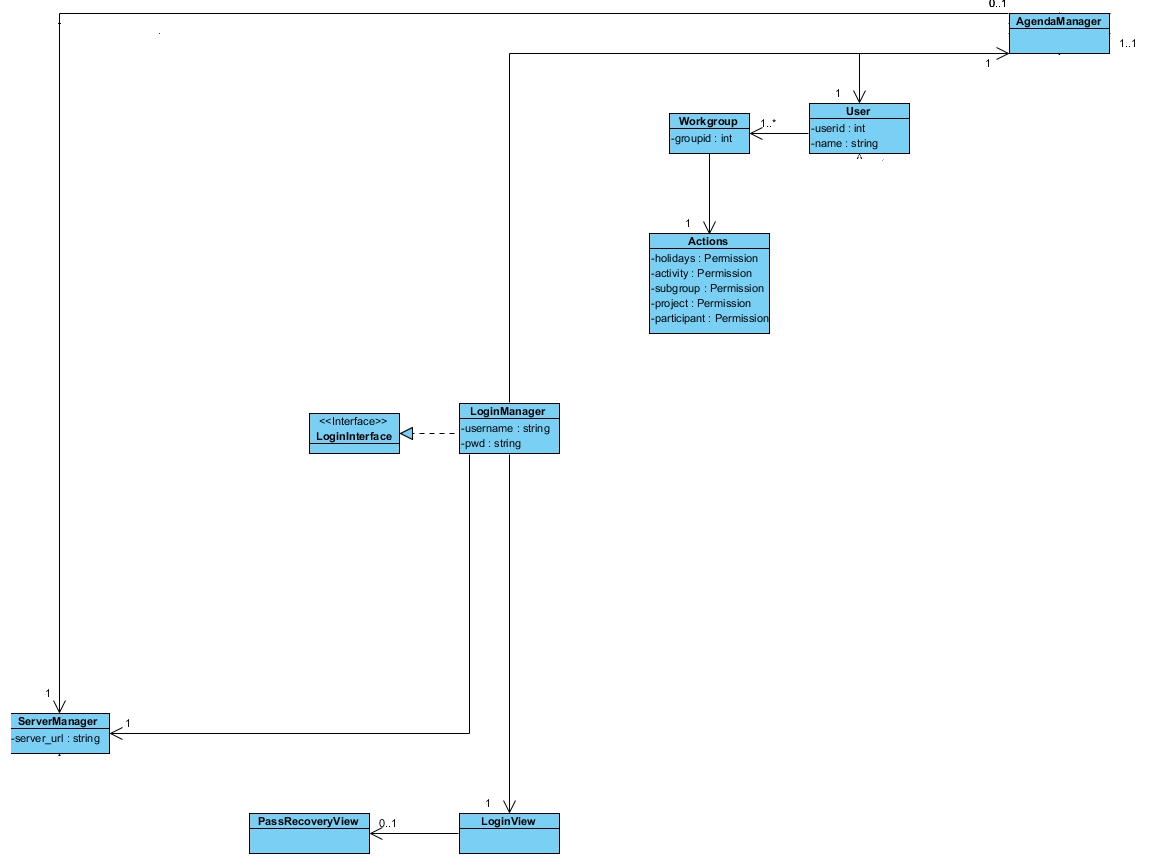
\includegraphics[scale=0.45]{4.png}

In particolare il sistema di Login dell'applicativo pu\`o essere personalizzato a
piacimento in base alle richieste di sicurezza o per semplificare l'accesso.
Lo stesso vale per i sistemi di Database che possono variare molto in base al tipo
di dati da salvare, alla mole di dati o alle preferenze dell'utente, generalizzando
una interfaccia d'accesso alle operazioni possiamo quindi suddividere il sistema
di storage dal suo utilizzo che rimane invariato dall'esterno.
\subsection{Diagrammi Completi}
Nelle pagine seguenti saranno mostrati (nell'ordine sottostante):
    \begin{itemize}
    \item Diagramma Casi d'Uso
    \item Diagramma Classi Client
    \item Diagramma Classi Implementato Client
    \item Diagramma di Sequenza di Login
    \item Diagramma Pacchetti
    \item Diagramma Classi Server
    \item Diagramma Classi Server implementato
    \item Diagramma Stati Client
    \end{itemize}
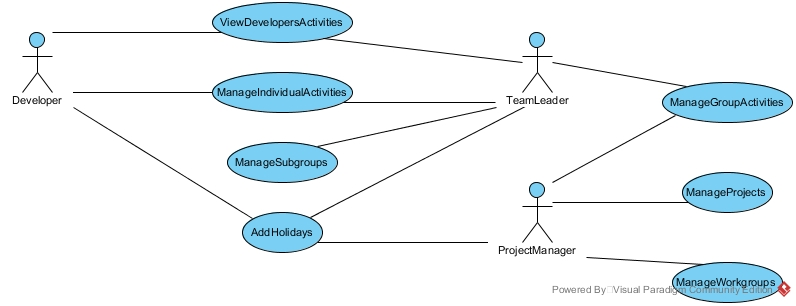
\includegraphics[angle=90,origin=c,scale=0.7]{ManageIT_UseCase.jpg}\\
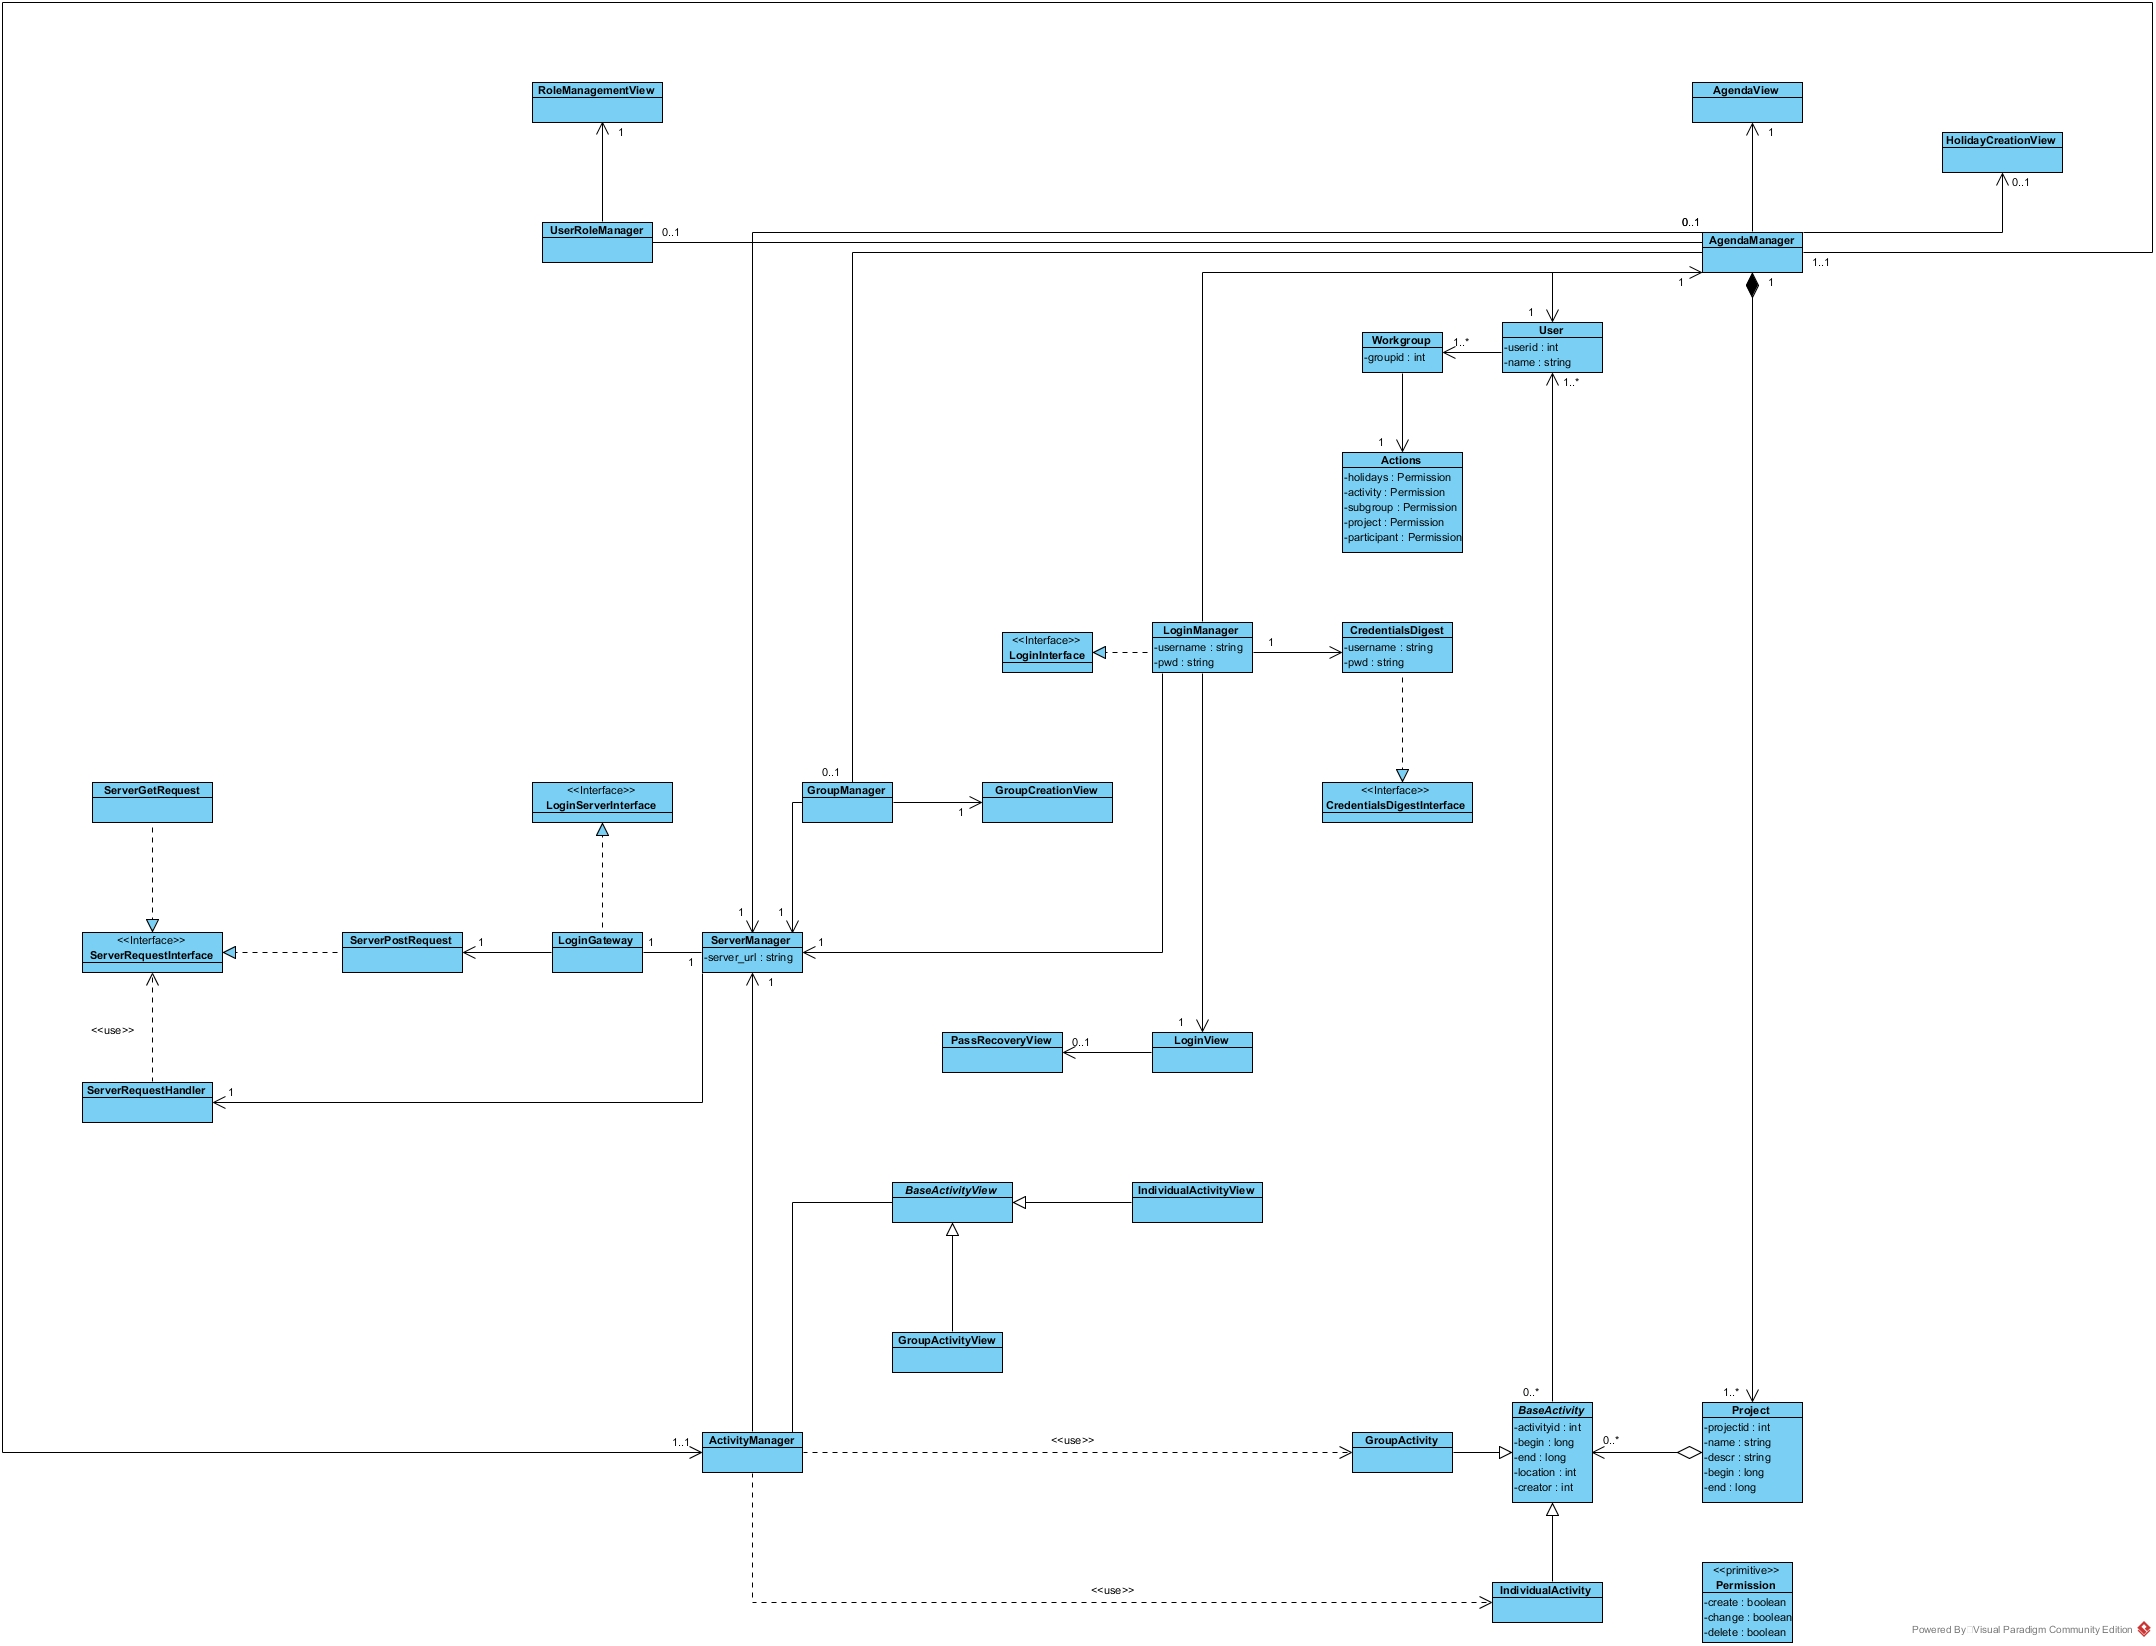
\includegraphics[angle=90,origin=c,scale=0.45]{ManageIT_Client_DomainClassDiagram.jpg}\\
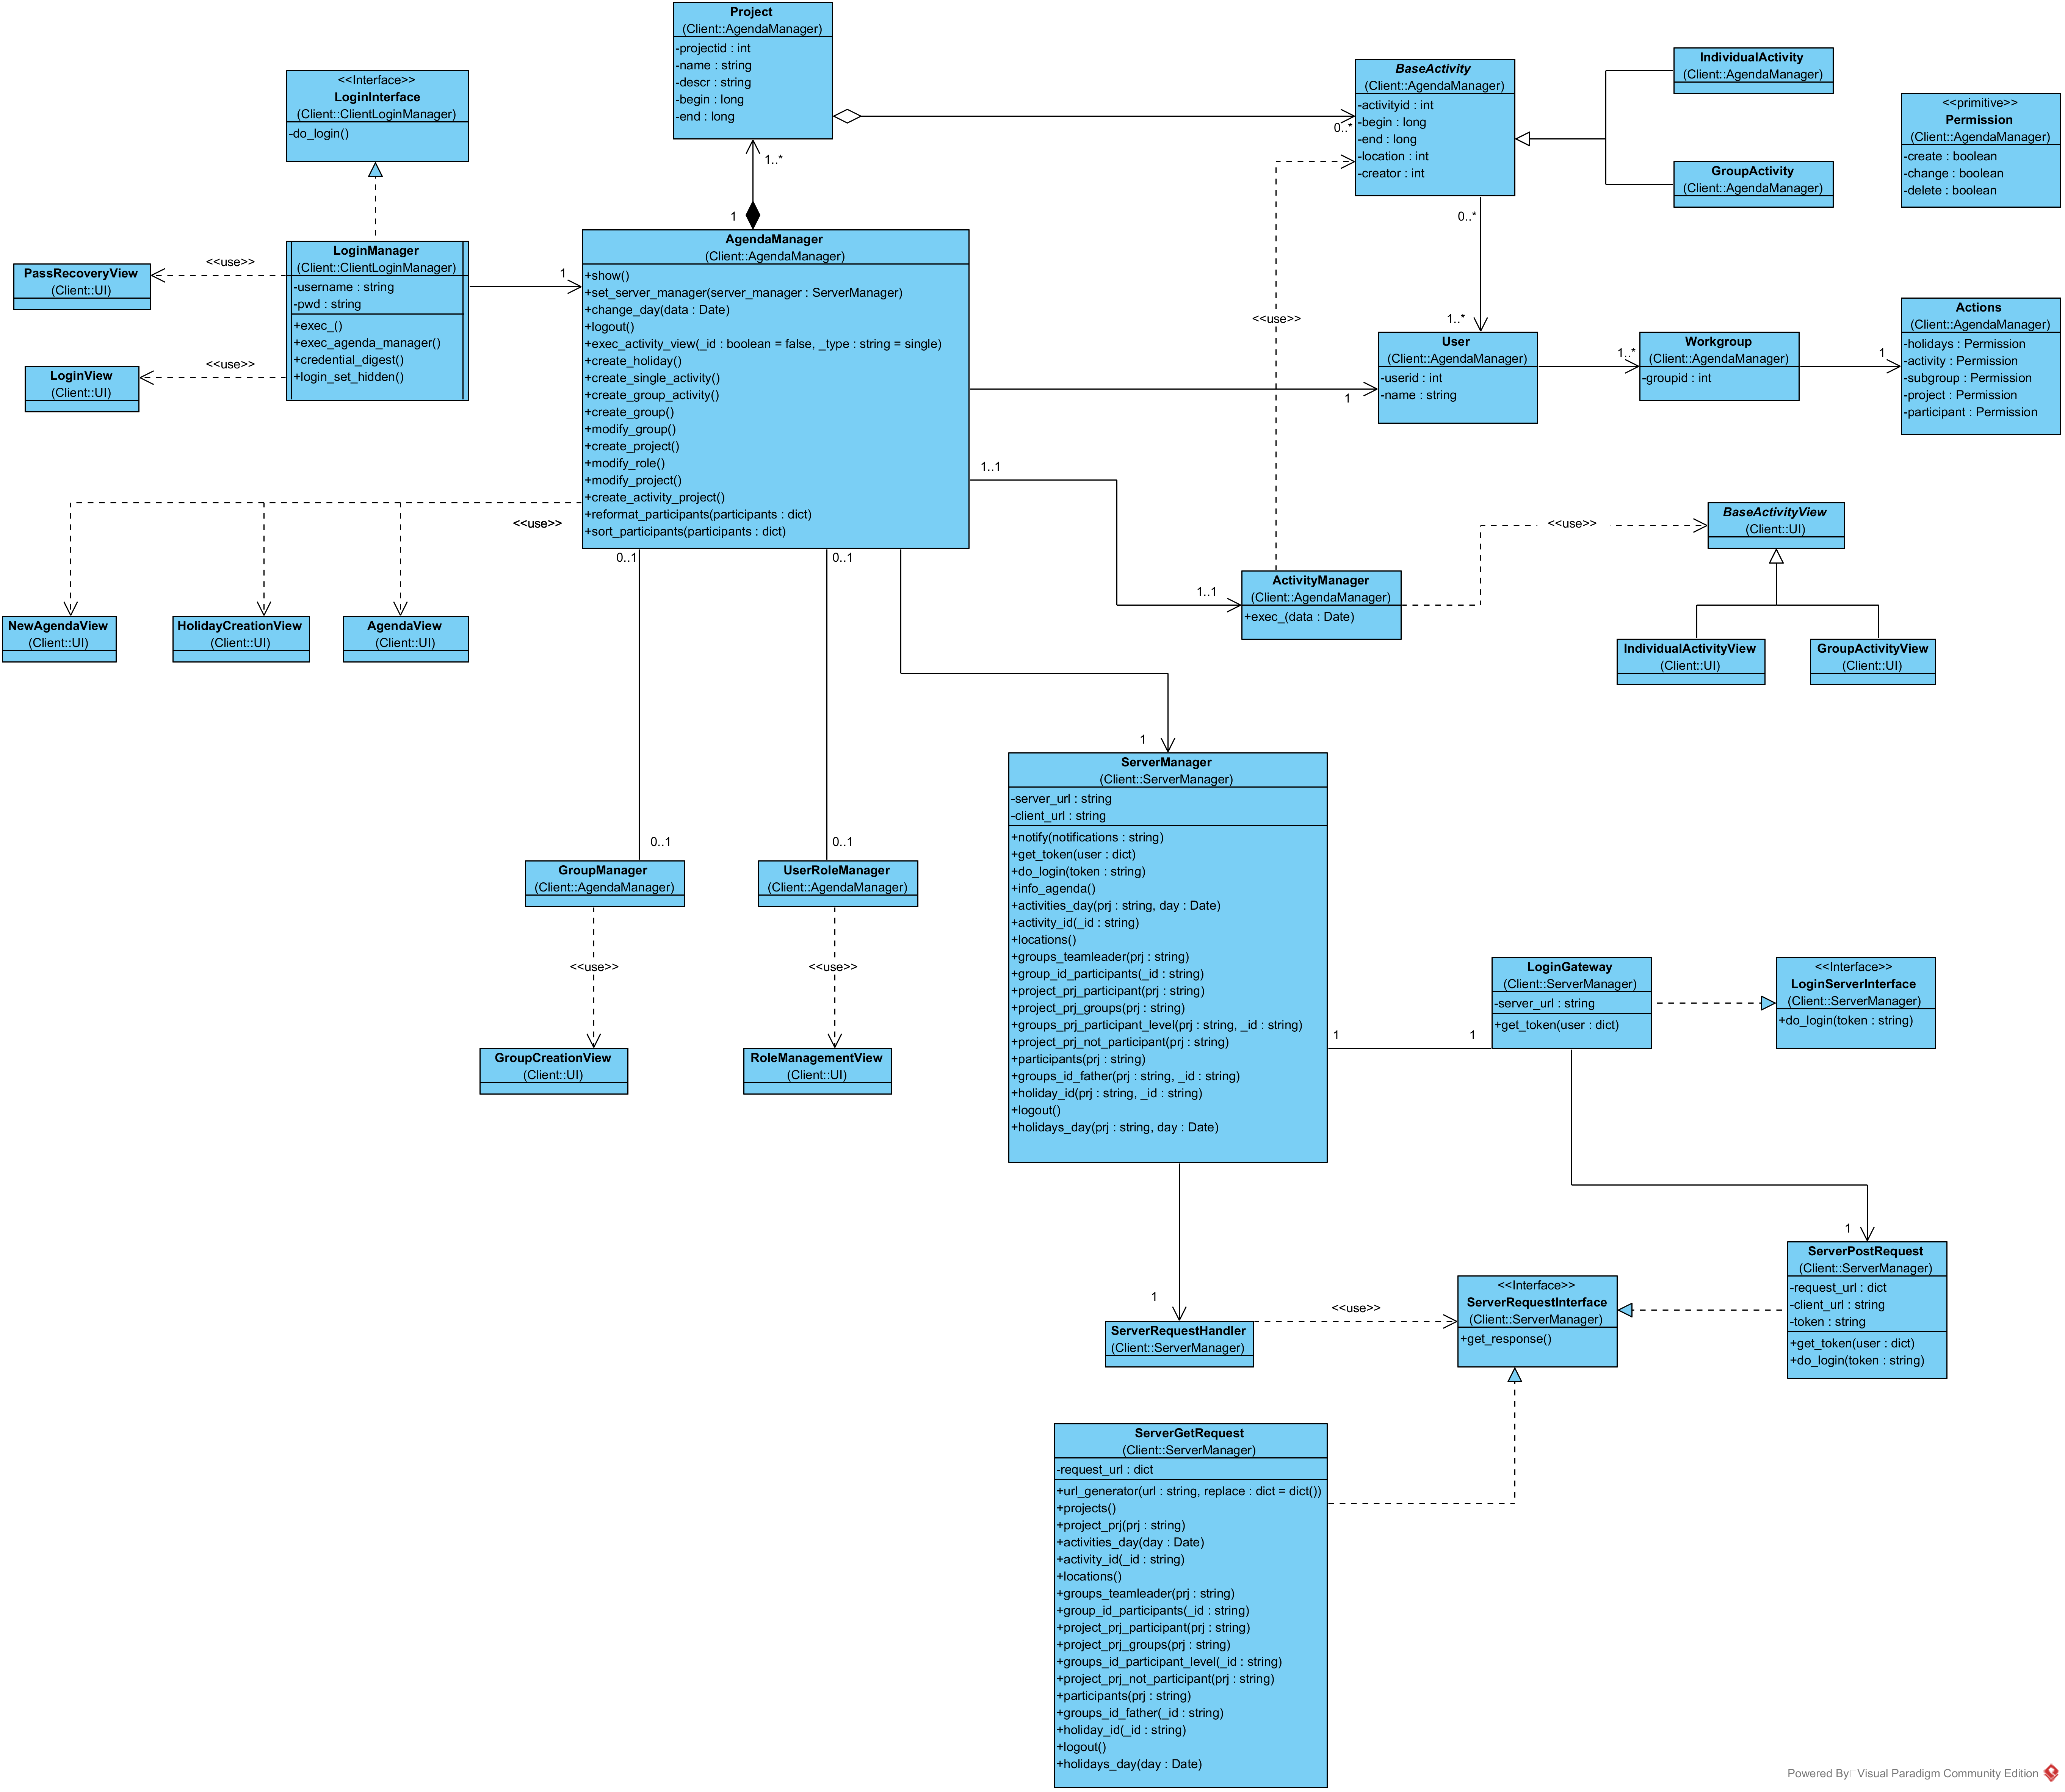
\includegraphics[scale=0.4]{ManageIT_Client_ImplementedClassDiagram.png}\\
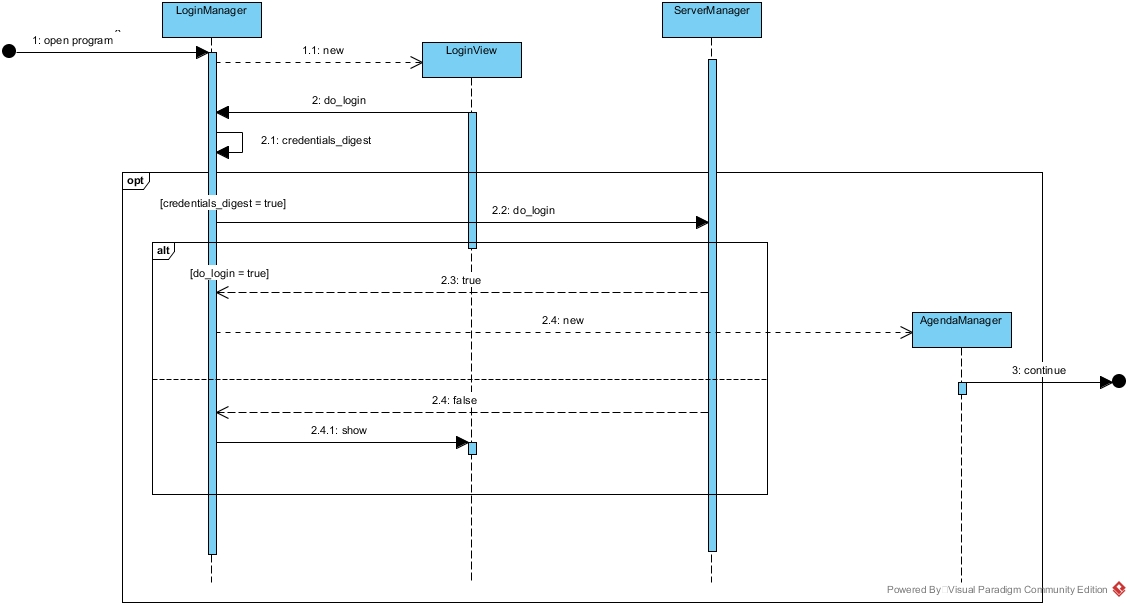
\includegraphics[angle=90,origin=c,scale=0.6]{ManageIT_LoginSequenceClasses.jpg}\\
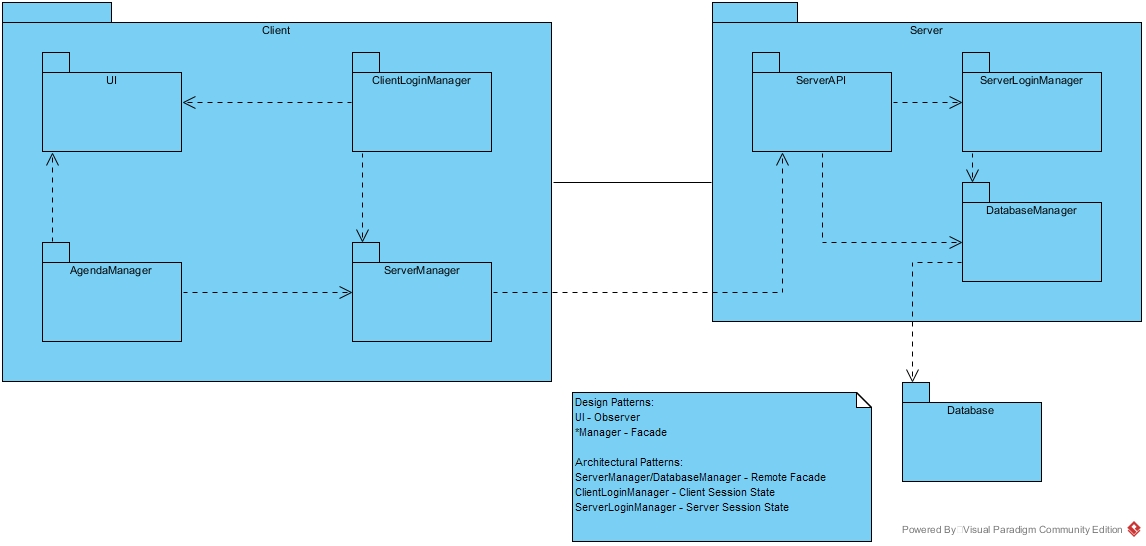
\includegraphics[angle=90,origin=c,scale=0.6]{ManageIT_PackageDiagram.jpg}\\
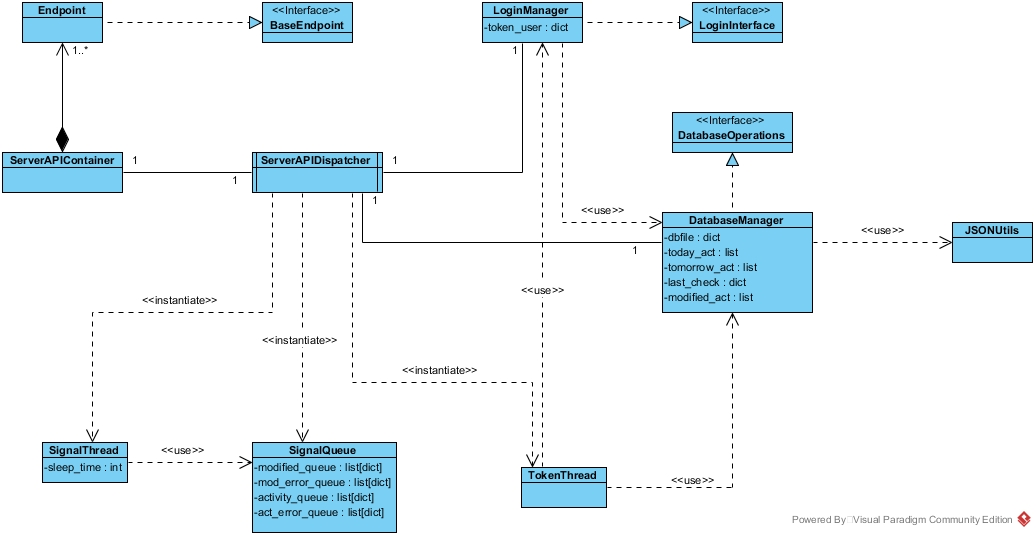
\includegraphics[angle=90,origin=c,scale=0.6]{ManageIT_Server_DomainClassDiagram.jpg}\\
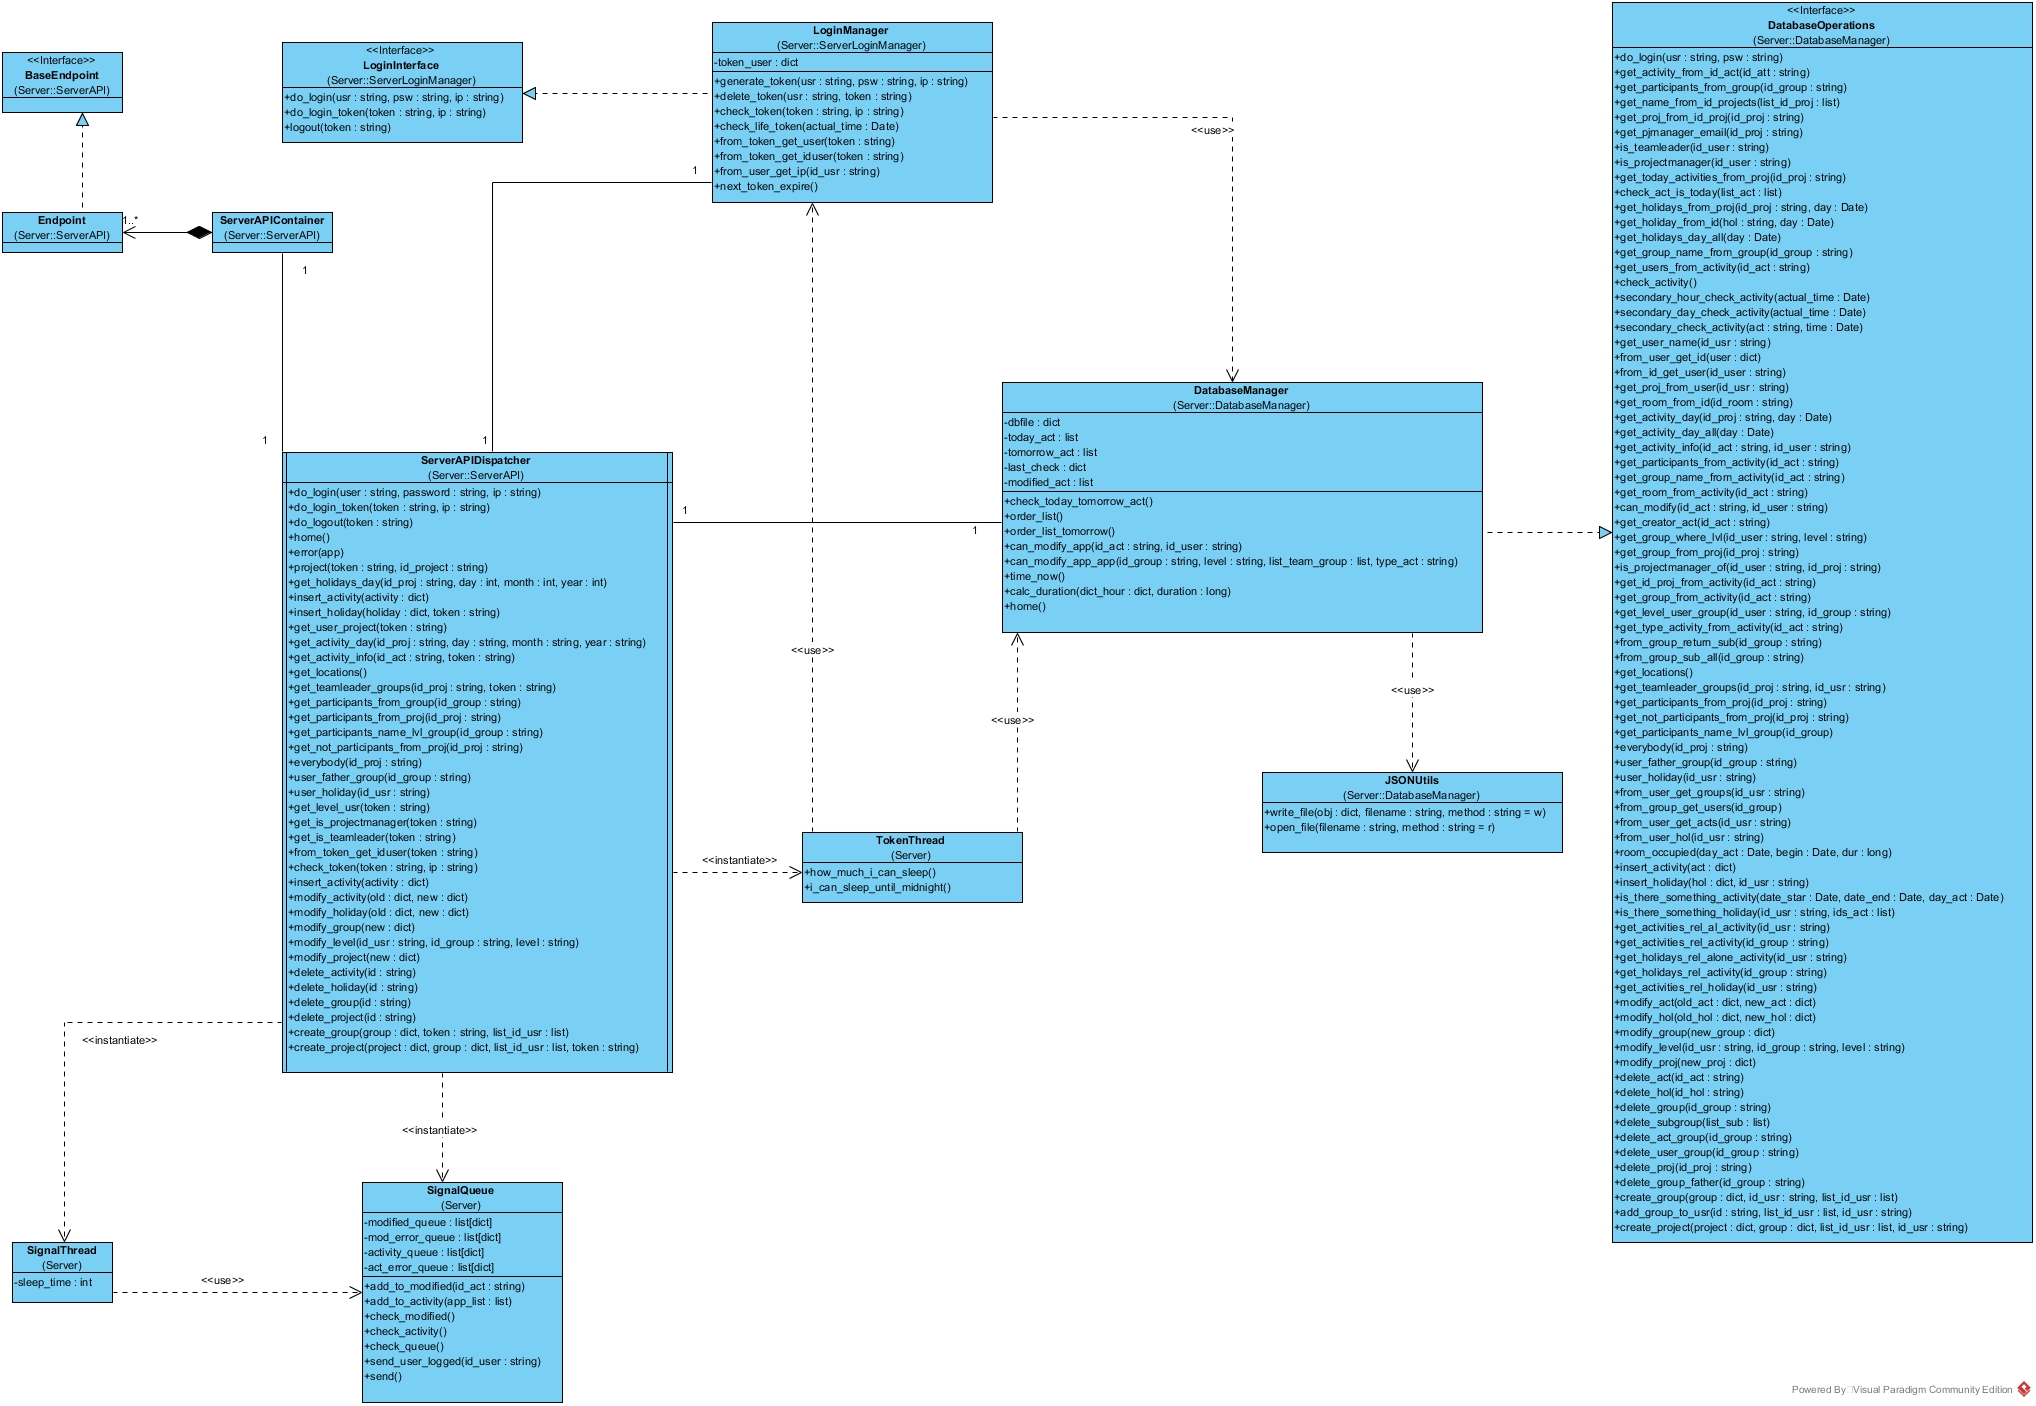
\includegraphics[angle=90,origin=c,scale=0.37]{ManageIT_Server_ImplementedClassDiagram.jpg}
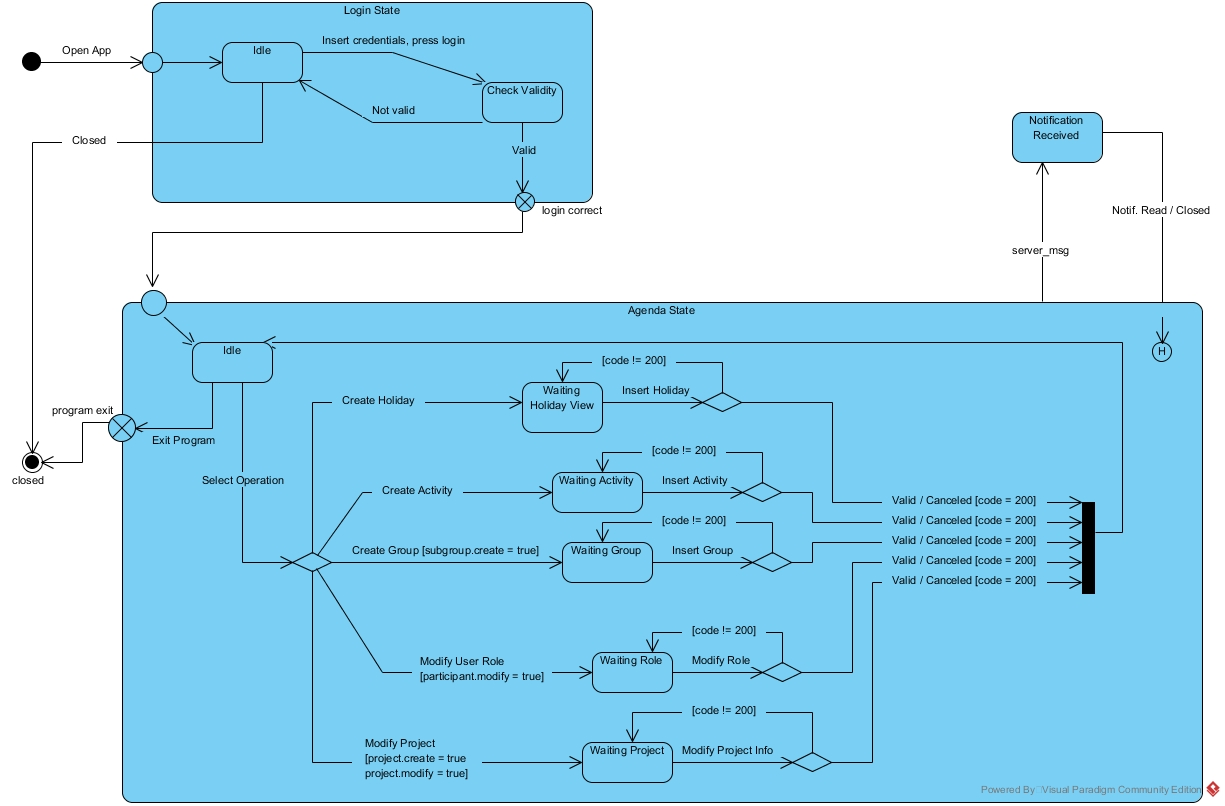
\includegraphics[angle=90,origin=c,scale=0.6]{ManageIT_StateChart_Client.jpg}

\end{document}
